\subsection{Benchmarks and Test Data}

\ifPresentation
%%%%%%%%%%%%%%%%%%%%%%%%%%%%%%%%%%%%%%%%%%%%%%%%%%%%%%%%%%
\begin{frame}[t]{Benchmarks}

    \justifying
    
    \begin{itemize}
        \setlength\itemsep{0.5cm}
        
        \item \textbf{Testing} of new concepts and ideas directly \text{in ATHLET} can be quite:
        \begin{itemize}
            \item cumbersome
            \item computationally expensive
            \item inconvenient
        \end{itemize}
        
        \item Therefore, two dedicated benchmarks have been developed:
            \begin{enumerate}
                \item \textbf{BM1}: tests \textbf{only} data \textbf{accumulation} i.e. uses \textbf{MPI\_Bcast}
                
                \item \textbf{BM2}: tests \textbf{both} data accumulation and non-blocking data transfer i.e. uses \textbf{MPI\_Ibcast}
            \end{enumerate}
            
        \item The benchmarks fully replicates all \textbf{basic ideas} of ATHLET
        
        \item Column vectors are generated \textbf{without} compute-expensive \textbf{function evaluations} i.e. filled with random numbers
    \end{itemize}

\end{frame}


%%%%%%%%%%%%%%%%%%%%%%%%%%%%%%%%%%%%%%%%%%%%%%%%%%%%%%%%%%
\begin{frame}[t]{Test Data and Process Allocation}

    \justifying
    \small
   
     \begin{figure}[t]
        \centering
        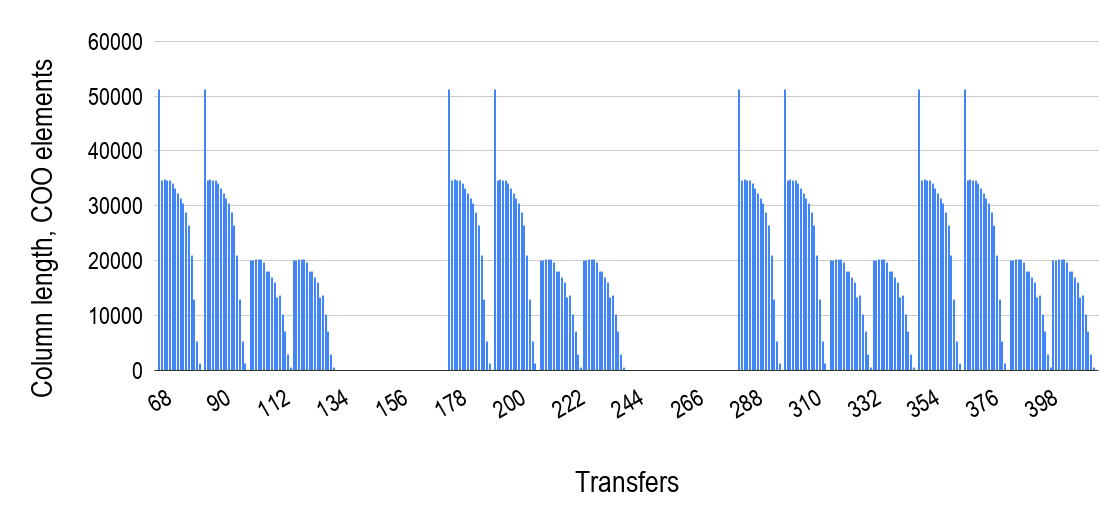
\includegraphics[width=0.6\textwidth]{figures/chapter-3/communication-pattern.png}
        \caption{A part of \textbf{cube-64} communication pattern}
    \end{figure}

    \vspace{-20.0pt}
    \begin{itemize}
        \item \textbf{Patterns} of the most common GRS simulations were \textbf{recorded}
    
        \item The recordings were \textbf{played inside} of the benchmarks
    
        \item The recordings were used \textbf{to generate} dummy column arrays
    
        \item Tested for \textbf{intra-socket, intra-node and inter-node} communication
    
    \end{itemize}

\end{frame}
\fi

\ifSpeech
%%%%%%%%%%%%%%%%%%%%%%%%%%%%%%%%%%%%%%%%%%%%%%%%%%%%%%%%%%
\begin{frame}[t]{Test Data}
    \justifying
    \begin{itemize}
        \item Communication \textbf{patterns were recorded} while ATHEL was executing some common GRS simulations
        
        \item The recordings were used \textbf{to generate} the corresponding column vector \textbf{lengths}
        
        \item The recordings were \textbf{played inside} of the benchmarks
    \end{itemize}
    
    \begin{figure}[htpb]
        \centering
        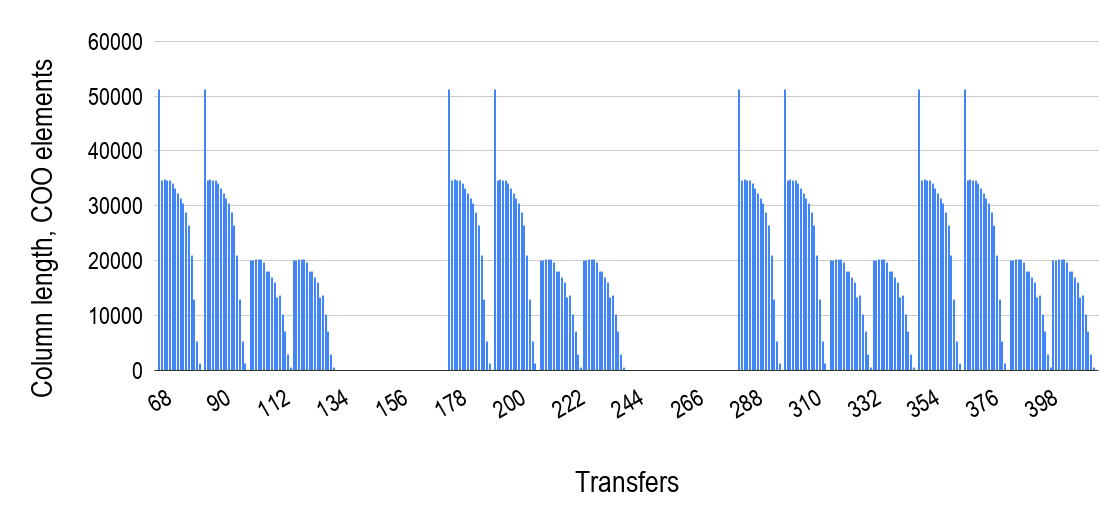
\includegraphics[width=0.7\textwidth]{figures/chapter-3/communication-pattern.png}
        \caption{A part of \textbf{cube-64} communication pattern} \label{fig:communication-pattern}
    \end{figure}

\end{frame}



%%%%%%%%%%%%%%%%%%%%%%%%%%%%%%%%%%%%%%%%%%%%%%%%%%%%%%%%%%
\begin{frame}[t]{Client-Server Process Allocation}
    \small
    \justifying
    
    \begin{itemize}
        \item \text{Three} process allocation \textbf{schemes} were tested on \textbf{HW1 cluster}:
        \begin{itemize}
            \item \textbf{intra-socket} i.e. client and server are distributed within the same socket
            \item \textbf{intra-node} i.e. client and server are distributed among different sockets of the same node
            \item \textbf{inter-node} i.e. client and server are distributed among different nodes
        \end{itemize}
    \end{itemize}

    \begin{figure}[t]
        \centering
        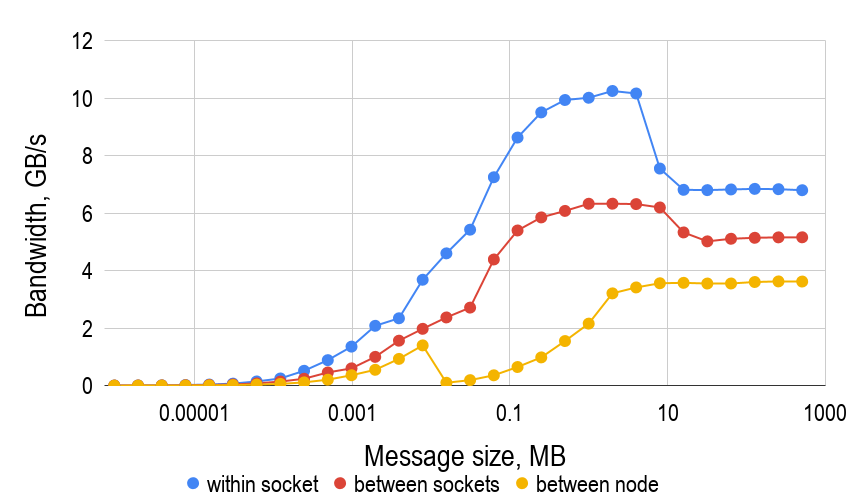
\includegraphics[width=0.55\textwidth]{figures/chapter-3/hw1-bandwidth.png}
    \end{figure}

\end{frame}
\fi